\section{Zielsetzung}
In diesem Versuch soll der effektive Dämpfungswiderstand
einer gedämpften Schwingkreisschaltung als auch beim aperiodischen Grenzfall
untersucht und ermittelt werden. Ebenso wird die Frequenzabhängigkeit
der Kondensatorspannung und die Phasenverschiebung von der außen gelegten Spannung
untersucht.
\section{Theorie}
Ein $CL$-Schwingkreis, das aus der Kapazität $C$ des Kondensators und der
Induktivität $L$ der Spule besteht, wird in der Physik durch den
Energieaustausch der beiden Baudelemente als eine periodische Schwingung bezeichnet.
Solange kein energieverbrauchendes Bauelement hinzukommt ist der Austausch unbegrenzt lang
und wird als ungedämpfte Schwingung bezeichnet.
Bei einer gedämpften Schwingung wird als energieverbrauchendes Bauelement ein ohmscher Widerstand $R$
hinzugeschaltet wie in Abbildung (\ref{fig:1}) zu sehen ist.
\begin{figure}[H]
\centering
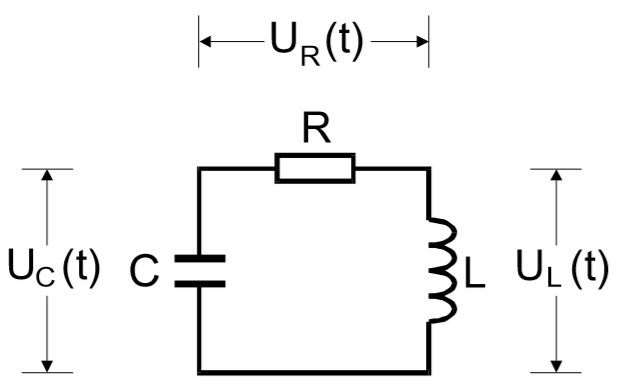
\includegraphics[width=\textwidth]{Schwingkreis.png}
\caption{Schaltdarstellung einer gedämpften Schwigung[1].}
\label{fig:1}
\end{figure}
Nun beginnt kein unendlicher Energieaustausch zwischen der Kapazität $C$
des Kondensators und der Induktivität $L$ der Spule statt.
Die Spannungen die an den einzelnen Bauelementen abfallen,
können mit Hilfe der Maschenregel, zu einer Differentialgleichung aufgestellt und umgeformt werden.
\begin{equation}
  \ddot{I} + \frac{R}{L} \cdot \dot{I} +\frac{1}{LC}\cdot I = 0
  \label{eq:1}
\end{equation}
Die Lösung der Gleichung (\ref{eq:1}) lautet:
\begin{equation}
  I(t) = A_1 \cdot e^{i\omega_1 t} + A_2 \cdot e^{i\omega_2 t}
  \label{eq:2}
\end{equation}
Dabei ist
\begin{equation*}
  \omega_{1,2} =  i \frac{R}{2L} \pm \sqrt{\frac{1}{LC} - \frac{R^2}{4L^2}}
\end{equation*}
Es werden nun 2 Fälle betrachtet.\\

Der erste Fall $\frac{1}{LC} \gg \frac{R^2}{4L^2}$ folgt, dass $\omega$ reell ist.\\
Somit wird die Gleichung(\ref{eq:2}) mit Hilfe der Eulerschen Form zu
\begin{equation}
  I(t) = A_0 \cdot e^{-2\pi\mu t} \cdot cos(2\pi\nu t + \varphi)
\end{equation}
umgeschrieben. Dabei ist
\begin{align*}
    \mu = \frac{R}{4\pi L} \\
    \nu = \frac{1}{2\pi} \sqrt{\frac{1}{LC} - \frac{R^2}{4L^2}}
\end{align*}

Der zweite Fall $\frac{1}{LC} \ll \frac{R^2}{4L^2}$ folgt daraus, dass $\omega$ imaginär ist
und somit sich
\begin{equation*}
I(t) \sim e^{-(2\pi \mu - i 2 \pi \nu)t}
\end{equation*} verhält.\\
Ein Spezial Fall ist, wenn $\frac{1}{LC} = \frac{R^2}{4L^2}$ folgt daraus das der aperiodische Grenzfall eintrifft
und der Strom am schnellsten gegen null geht.
\newpage
Erzwungene Schwingungen werden mit einer Sinusspannung, wie in Abbildung(\ref{fig:2}) dargestellt, erzeugt.
\begin{figure}[H]
\centering
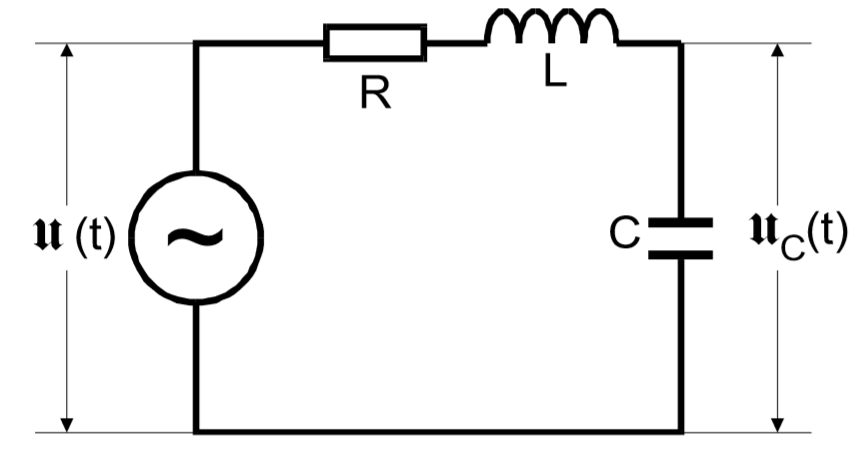
\includegraphics[width=\textwidth]{Schwingkreis2.png}
\caption{Schaltdarstellung einer erzwungene Schwinung[1].}
\label{fig:2}
\end{figure}

Dabei verändert sich die Gleichung (\ref{eq:1}) und die Lösung für solch eine Differentialgleichung lautet:
\begin{equation}
  U_c(\omega) = \frac{U_0}{\sqrt{(1-LC\omega^2 + (RC\omega)^2}}
  \label{eq:3}
\end{equation}
Die Phasenverschiebung zwischen der angelegten Sinusspannung und der Kondensatorspannung kann mit der Formel
\begin{equation}
\varphi(\omega) = \arctan(\frac{-\omega CR}{1-LC\omega^2})
\label{eq:4}
\end{equation}
errechnet werden.\\
Für $\omega \rightarrow \infty$ ist $U_c$ = 0 und für $\omega \rightarrow 0$ strebt $U_c$ gegen $U_o$.
Ab einer bestimmten Frequenz erreicht $U_c$
ein Maximum und ist größer als $U_o$.
Solch ein Phänomen bezeichnet man als Resonanz.
Die Resonanzfrequenz lässt sich mit der Formel
\begin{equation}
  \omega_{res} = \sqrt{\frac{1}{LC} - \frac{R^2}{2L^2}}
\end{equation}
 berechnen.
